\begin{figure}[ht!]
\centering
% manually adjust the width of the figure
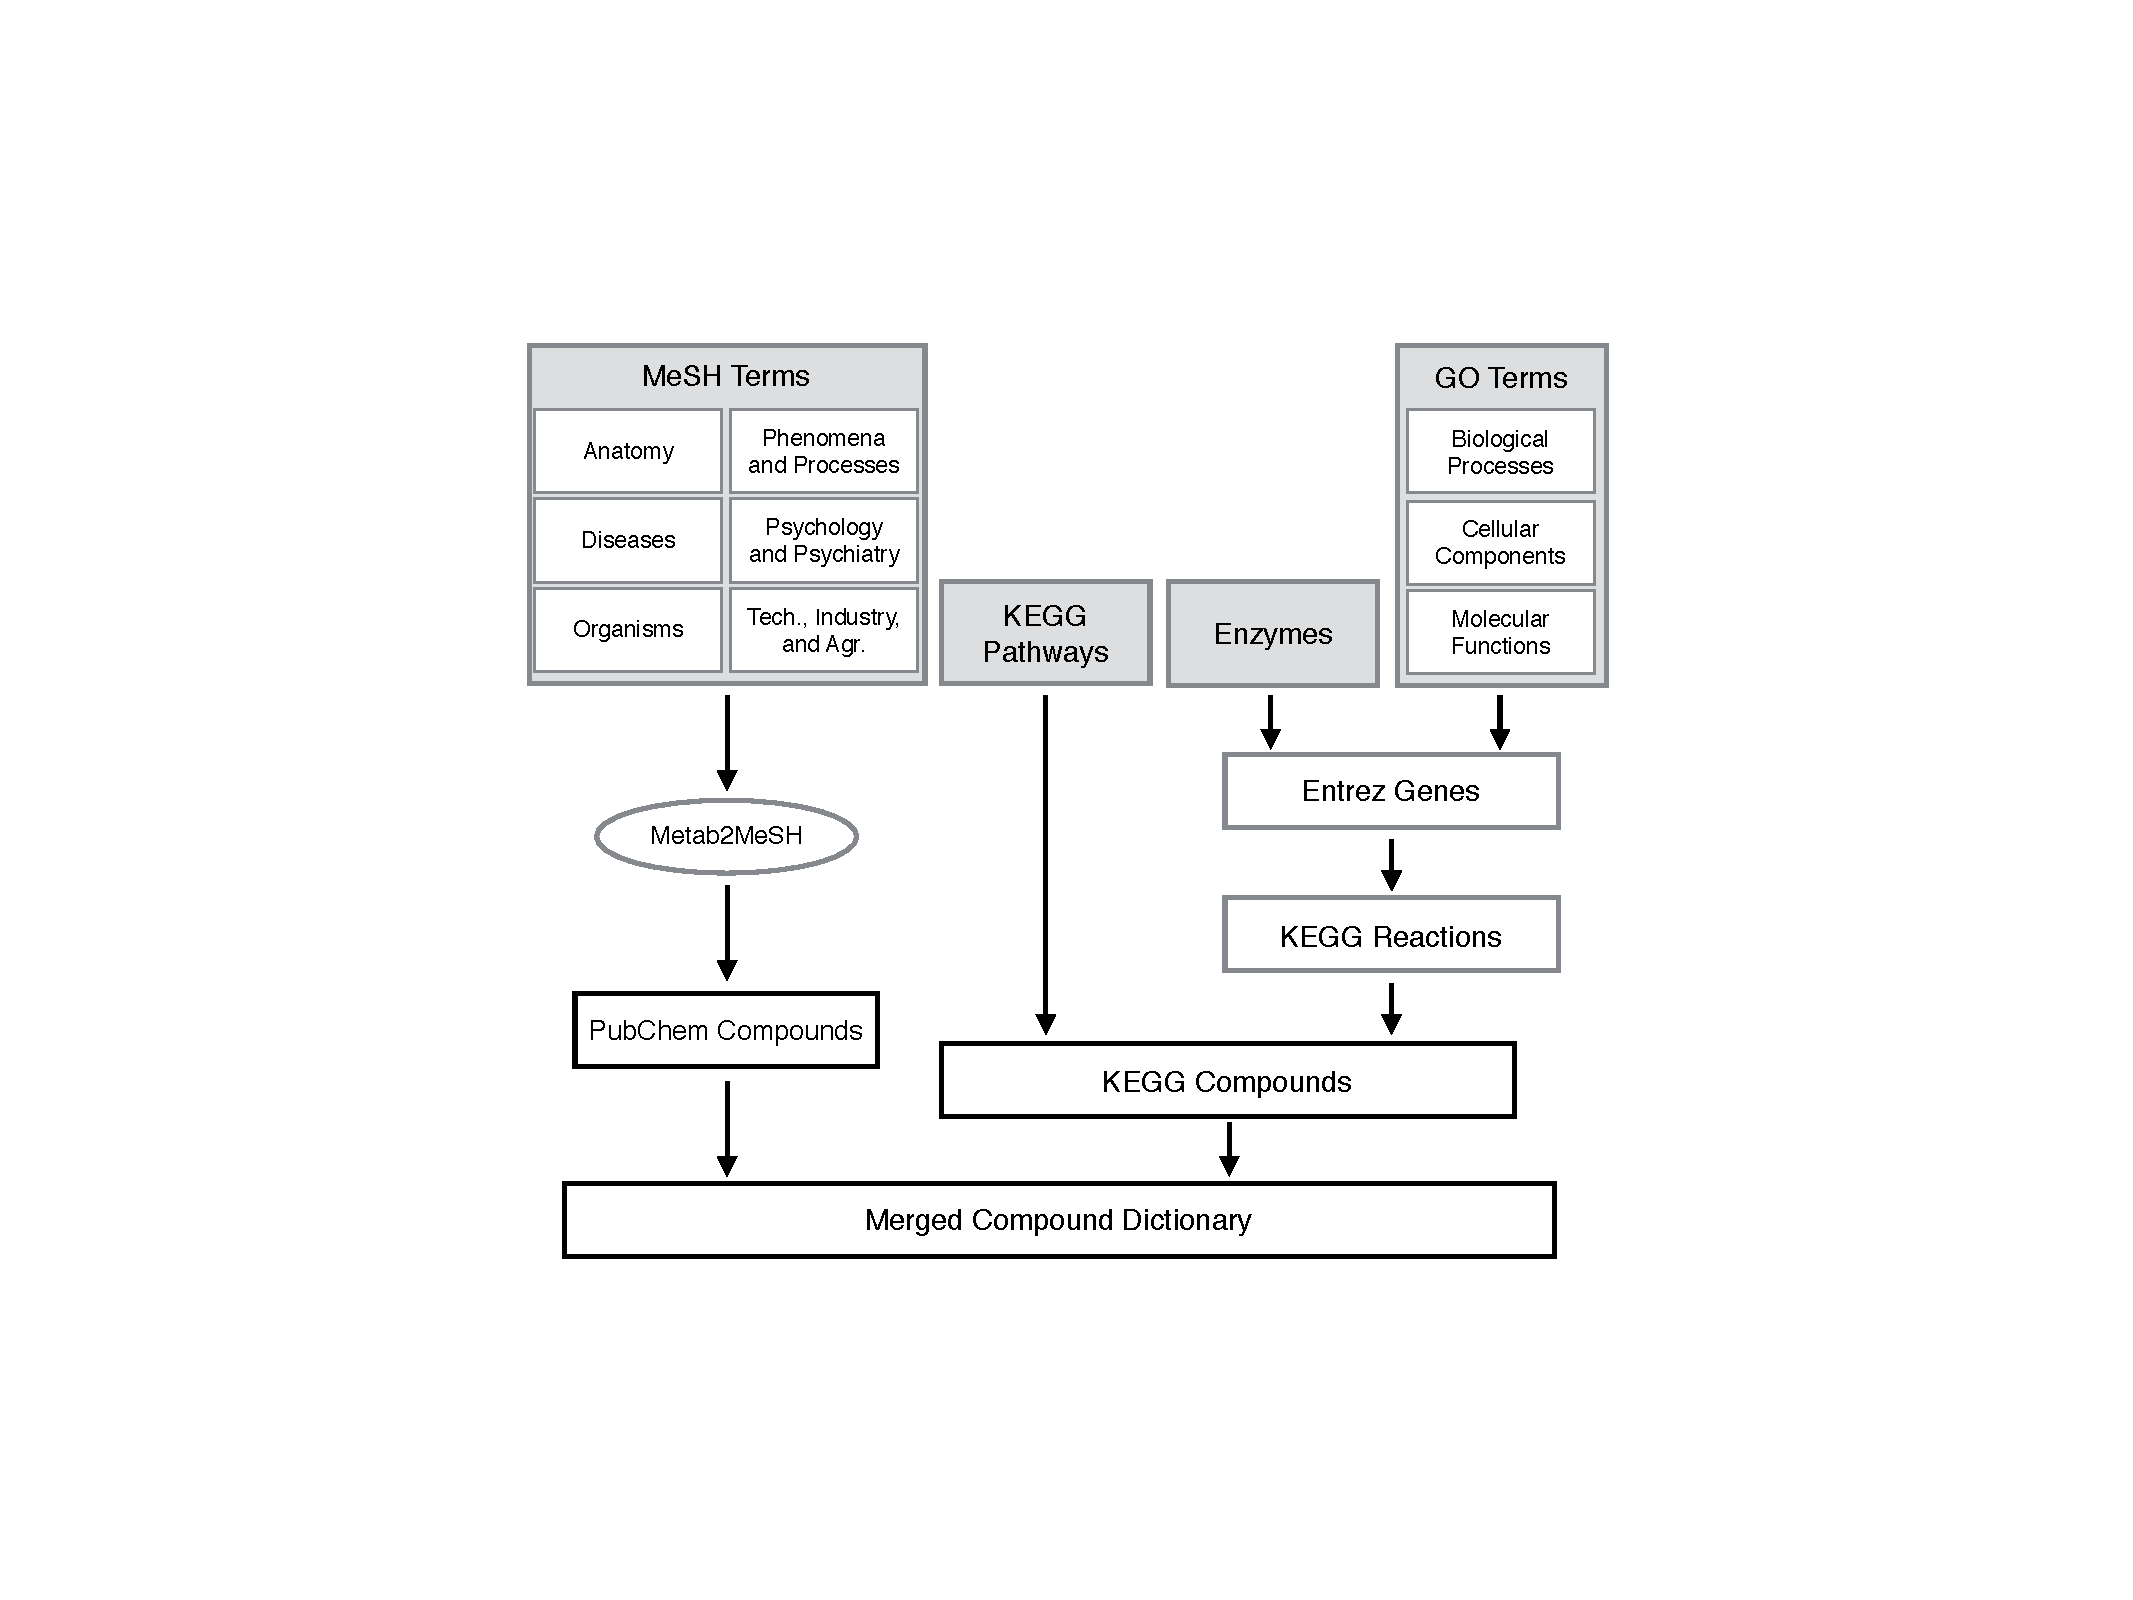
\includegraphics[width=1\textwidth]{chap3figs/figure3_1.pdf}
\caption[A diagrammatic view of how small molecules are annotated to concepts in ConceptMetab.]
{
% Rackham requires the figure list title matches the first sentence, so repeat that sentence here
\textbf{A diagrammatic view of how small molecules are annotated to concepts in ConceptMetab.} PubChem compounds are associated with MeSH Terms via Metab2MeSH. Metabolites with KEGG IDs are associated with KEGG Pathways via their XML representation. Enzymes and GO terms are mapped to KEGG compounds through Entrez genes and KEGG reactions. Finally, PubChem and KEGG small molecules are linked via a dictionary used in Metab2MeSH.
}
\label{chap3:fig:1}
\end{figure}

\newpage

\begin{figure}[ht!]
\centering
% manually adjust the width of the figure
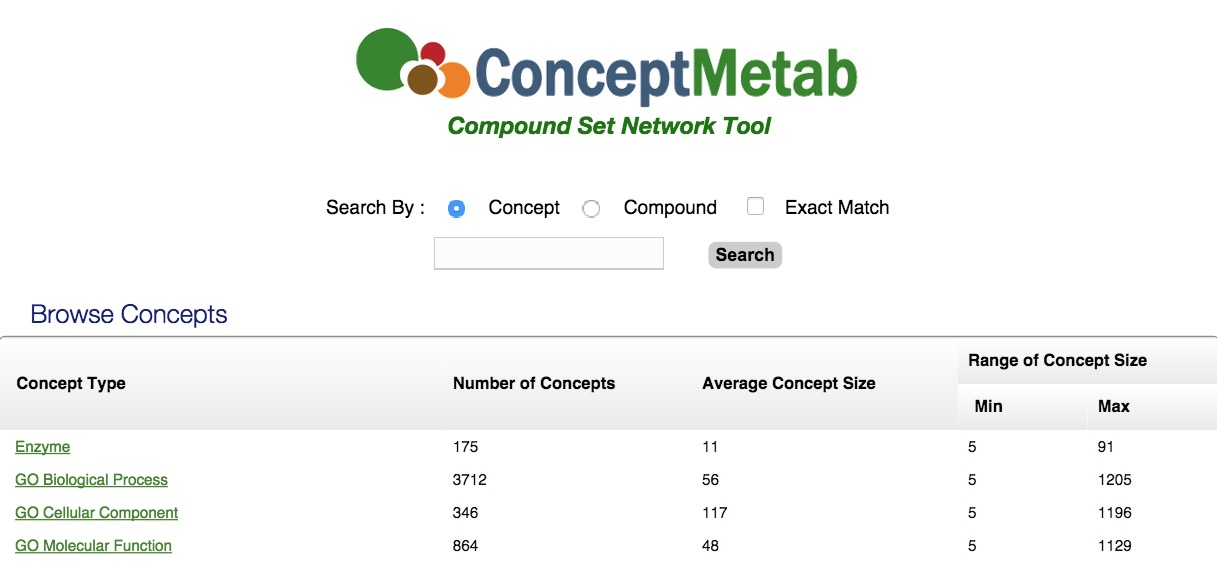
\includegraphics[width=1\textwidth]{chap3figs/figure3_2.jpg}
\caption[Searching in ConceptMetab.]
{
% Rackham requires the figure list title matches the first sentence, so repeat that sentence here
\textbf{Searching in ConceptMetab.} Users may search by biological concept or compound, or browse by concept type.
}
\label{chap3:fig:2}
\end{figure}

\newpage

\begin{figure}[ht!]
\centering
% manually adjust the width of the figure
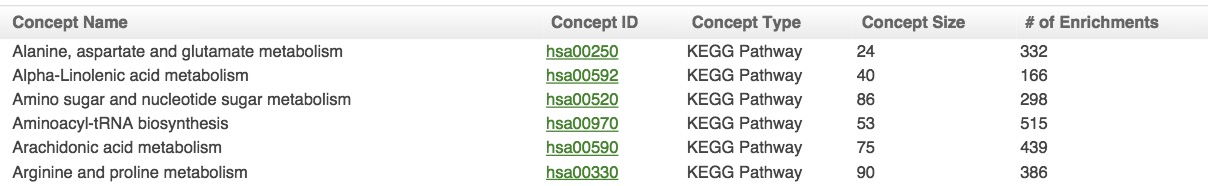
\includegraphics[width=1\textwidth]{chap3figs/figure3_3.jpg}
\caption[Browsing in ConceptMetab.]
{
% Rackham requires the figure list title matches the first sentence, so repeat that sentence here
\textbf{Browsing in ConceptMetab.} Browsing by concept type displays a list of biological concepts, their IDs from the originating database, the number of compounds in each concept, and the number of significantly associated concepts in ConceptMetab ($FDR < 0.05$).
}
\label{chap3:fig:3}
\end{figure}

\newpage

\begin{figure}[ht!]
\centering
% manually adjust the width of the figure
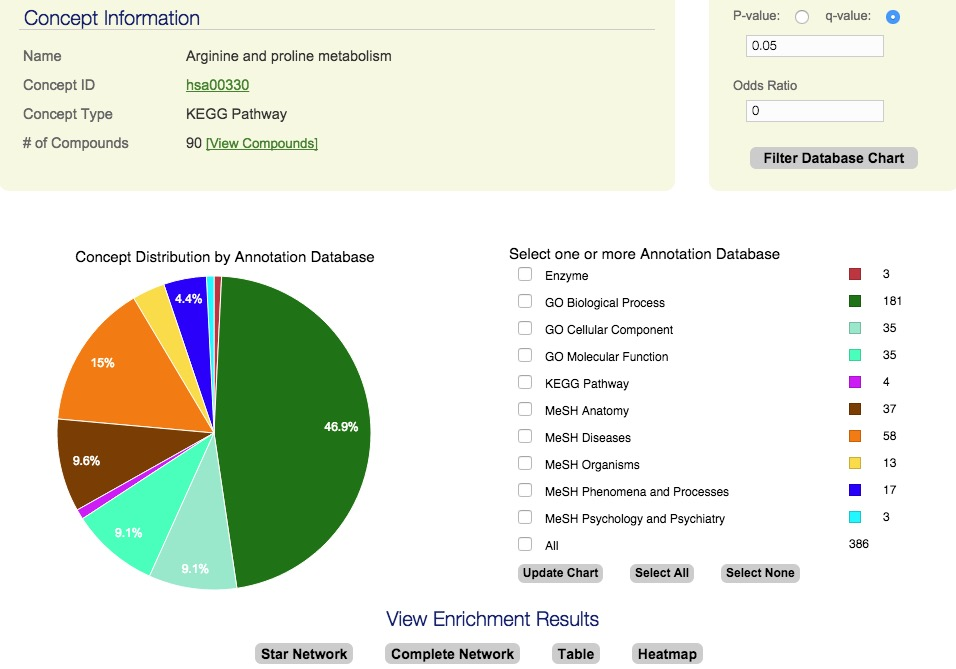
\includegraphics[width=1\textwidth]{chap3figs/figure3_4.jpg}
\caption[Concept overviews.]
{
% Rackham requires the figure list title matches the first sentence, so repeat that sentence here
\textbf{Concept overviews.} Selecting a concept displays an overview, including a summary of the concepts that are significantly associated with the chosen term. Users may alter the criteria for significance. Links are provided to the network visualizations, the enrichment table, and the heatmap.
}
\label{chap3:fig:4}
\end{figure}

\newpage

\begin{figure}[ht!]
\centering
% manually adjust the width of the figure
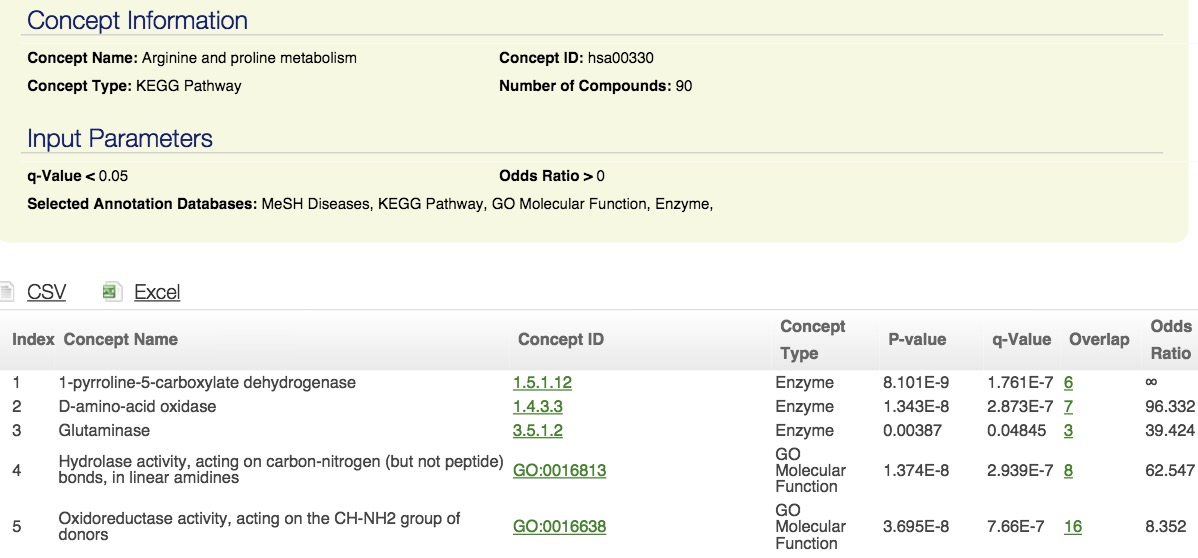
\includegraphics[width=1\textwidth]{chap3figs/figure3_5.jpg}
\caption[Enrichment results.]
{
% Rackham requires the figure list title matches the first sentence, so repeat that sentence here
\textbf{Enrichments results.} The enrichment table displays typical enrichment results with interactive links, and the ability to select individual concepts for inclusion in visualizations.
}
\label{chap3:fig:5}
\end{figure}

\newpage

\begin{figure}[ht!]
\centering
% manually adjust the width of the figure
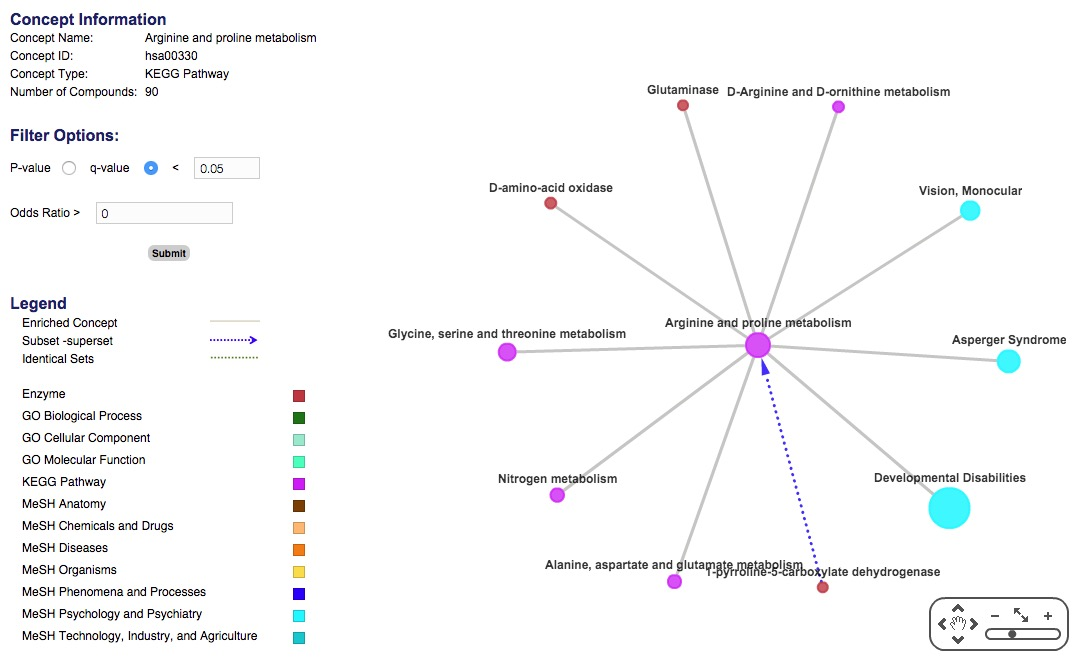
\includegraphics[width=1\textwidth]{chap3figs/figure3_6.jpg}
\caption[Star networks.]
{
% Rackham requires the figure list title matches the first sentence, so repeat that sentence here
\textbf{Star networks.} The star network visualizes concepts significantly associated with the concept. Color represents concept type and the size of node indicates the number of compounds. Clicking on a node displays concept information, and clicking an edge displays the compounds in common between the two concepts.
}
\label{chap3:fig:6}
\end{figure}

\newpage

\begin{figure}[ht!]
\centering
% manually adjust the width of the figure
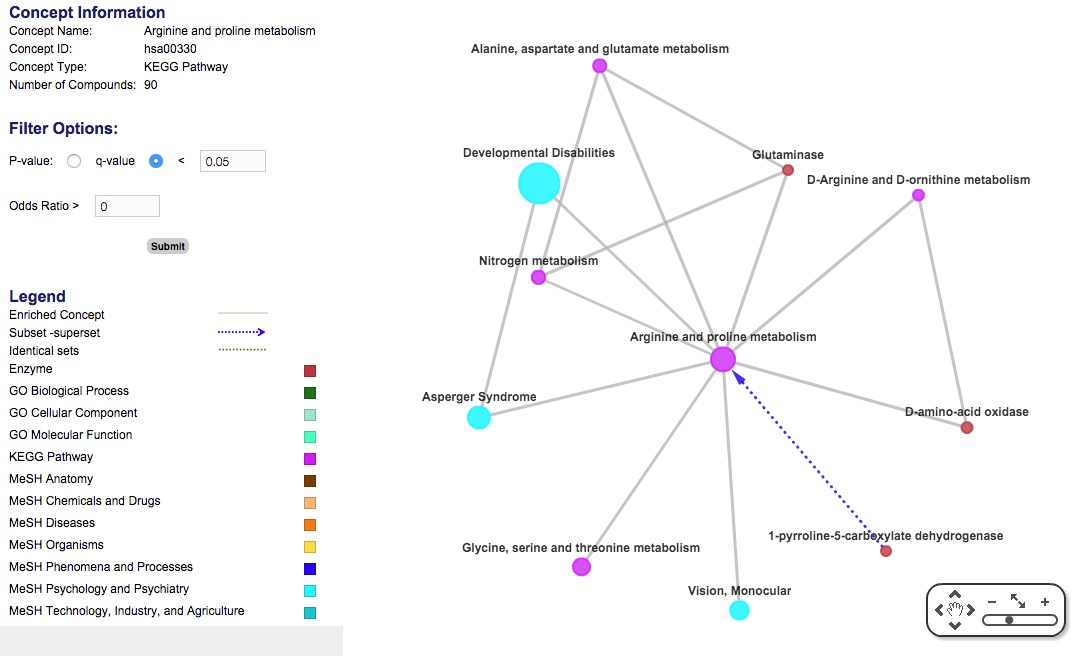
\includegraphics[width=1\textwidth]{chap3figs/figure3_7.jpg}
\caption[Complete networks.]
{
% Rackham requires the figure list title matches the first sentence, so repeat that sentence here
\textbf{Complete networks.} The complete network contains the same nodes as the star network, but also displays associations among the nodes.
}
\label{chap3:fig:7}
\end{figure}

\newpage

\begin{figure}[ht!]
\centering
% manually adjust the width of the figure
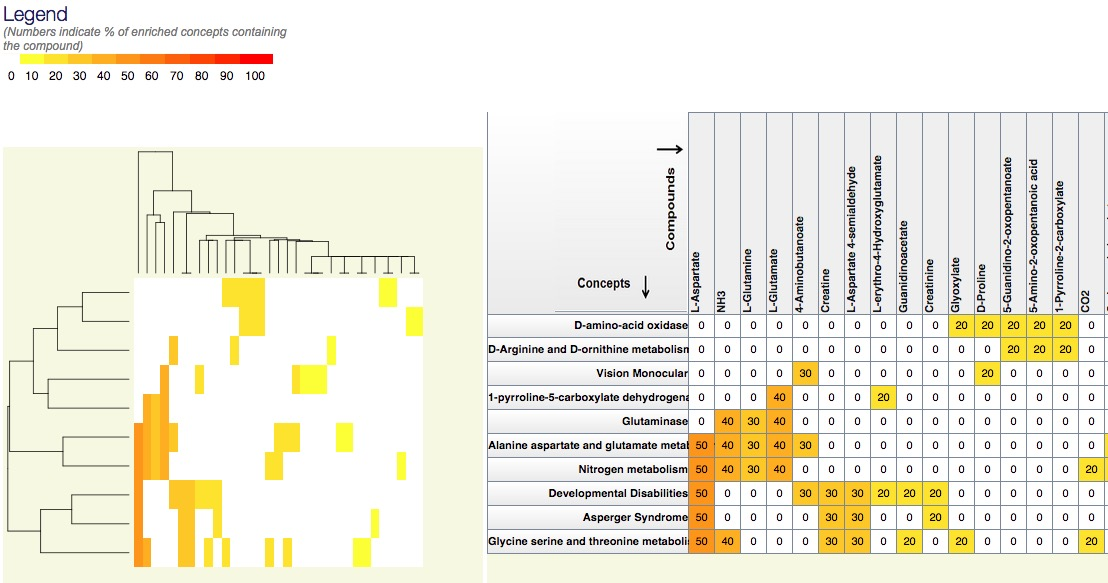
\includegraphics[width=1\textwidth]{chap3figs/figure3_8.jpg}
\caption[Heatmap.]
{
% Rackham requires the figure list title matches the first sentence, so repeat that sentence here
\textbf{Heatmap.} The heatmap allows users to investigate the compounds that are responsible for the observed associations. An overview heatmap image and an interactive version are provided.
}
\label{chap3:fig:8}
\end{figure}

\newpage

\begin{figure}[ht!]
\centering
% manually adjust the width of the figure
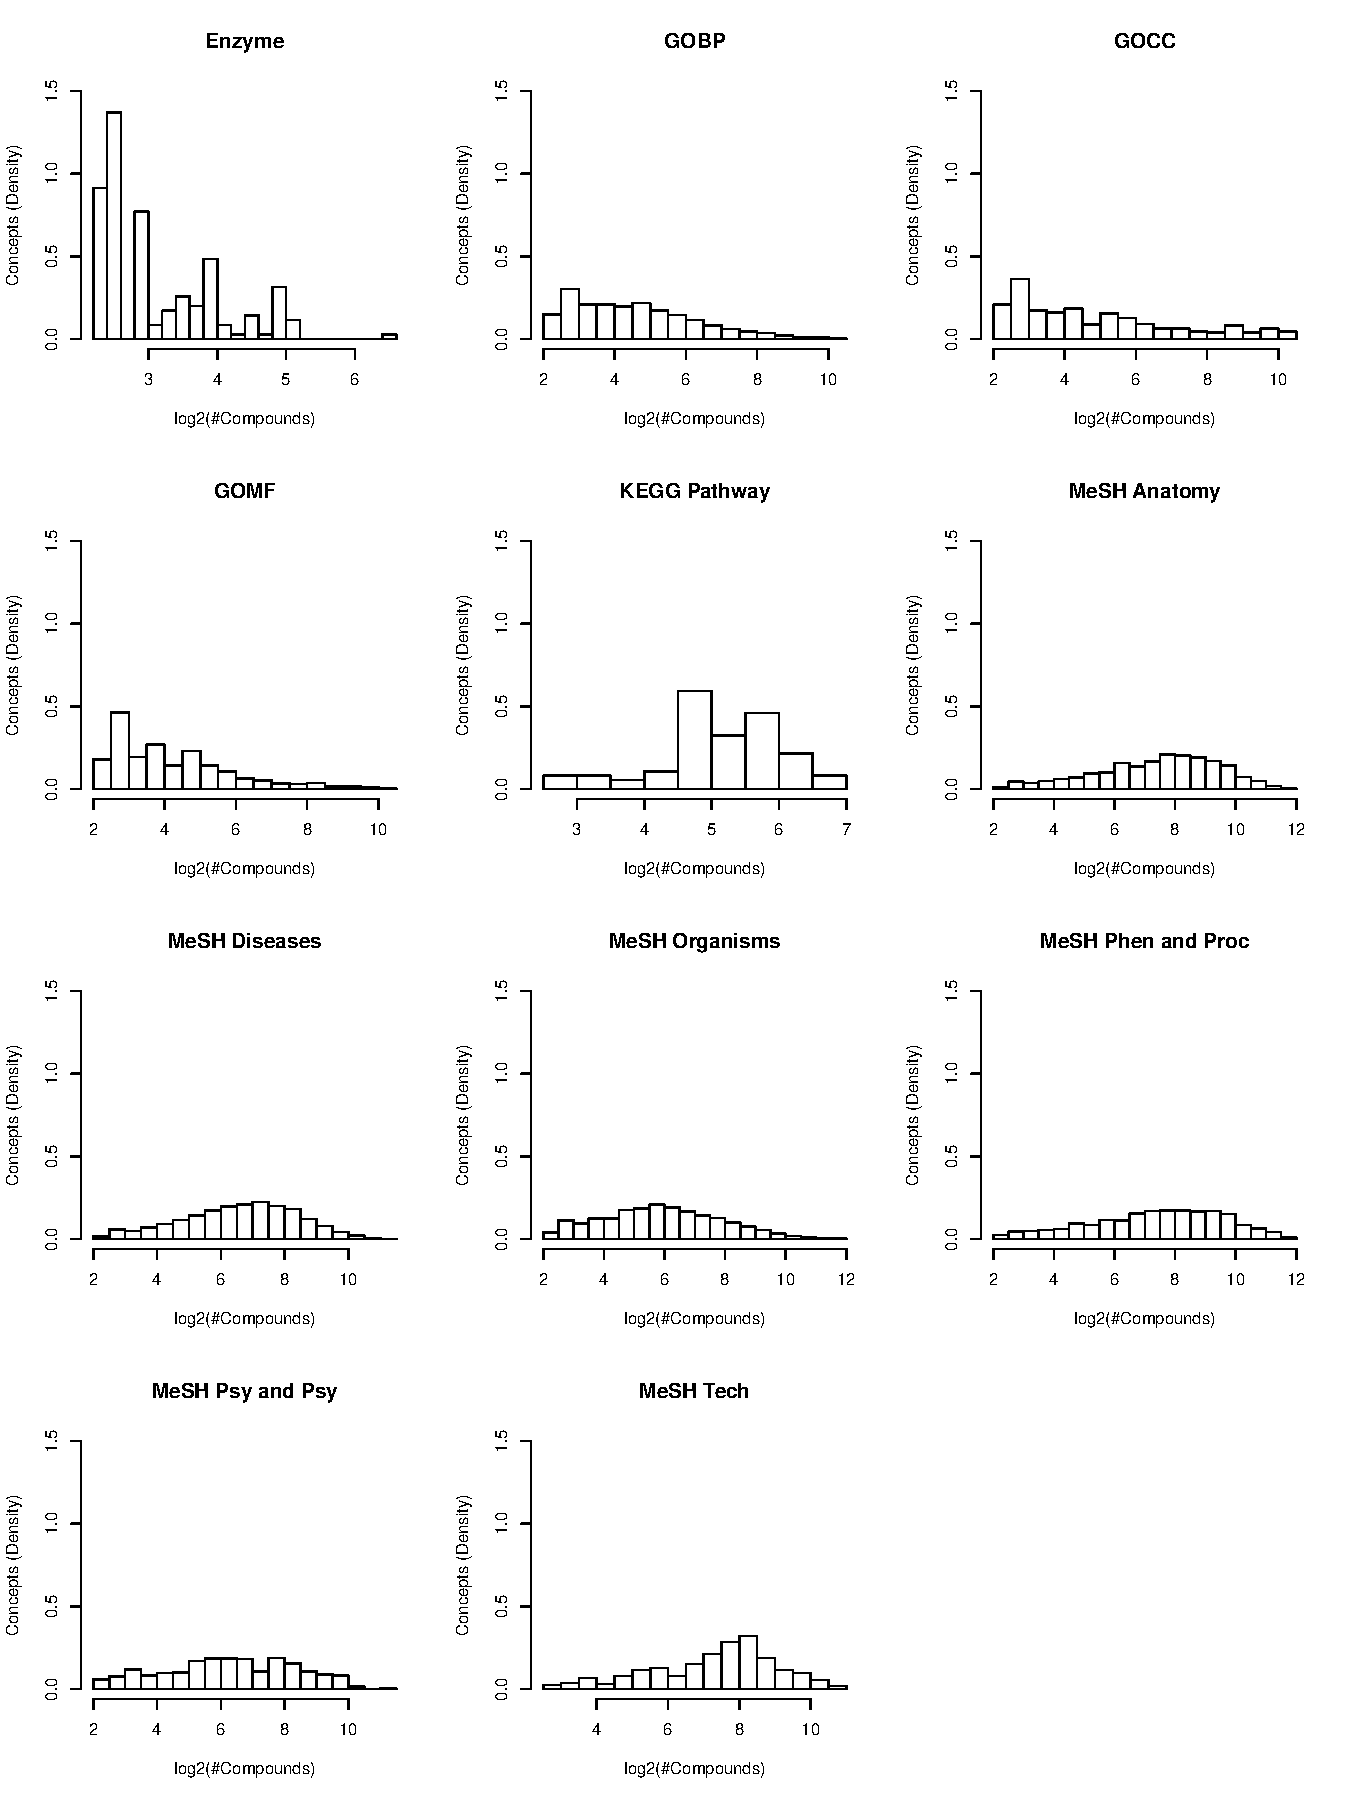
\includegraphics[width=1\textwidth]{chap3figs/figure3_10.pdf}
\caption[Distributions of the number of compounds per concept for each concept type.]
{
% Rackham requires the figure list title matches the first sentence, so repeat that sentence here
\textbf{Distributions of the number of compounds per concept for each concept type.} GOBP=Gene Ontology (GO) biological process; GOCC=GO cellular component; GOMF=GO molecular function.

}
\label{chap3:fig:9}
\end{figure}

\newpage

\begin{figure}[ht!]
\centering
% manually adjust the width of the figure
\includegraphics[width=1\textwidth]{chap3figs/figure3_9.pdf}
\caption[Distributions of the number of concepts per compound for each concept type.]
{
% Rackham requires the figure list title matches the first sentence, so repeat that sentence here
\textbf{Distributions of the number of concepts per compound for each concept type.}

}
\label{chap3:fig:10}
\end{figure}

\newpage

\begin{figure}[ht!]
\centering
% manually adjust the width of the figure
\includegraphics[width=1\textwidth]{chap3figs/figure3_11.pdf}
\caption[Proportion of enrichments between concept types.]
{
% Rackham requires the figure list title matches the first sentence, so repeat that sentence here
\textbf{Percentage of enrichments between concept types.} Numbers in each cell are the percentage of enrichment tests between the respective concept types which were significant ($FDR < 0.05$). Observe that KEGG-based concepts tend to be more enriched with other KEGG-based concepts, and similarly for PubChem-based concepts.
}
\label{chap3:fig:11}
\end{figure}

\newpage

\begin{figure}[ht!]
\centering
% manually adjust the width of the figure
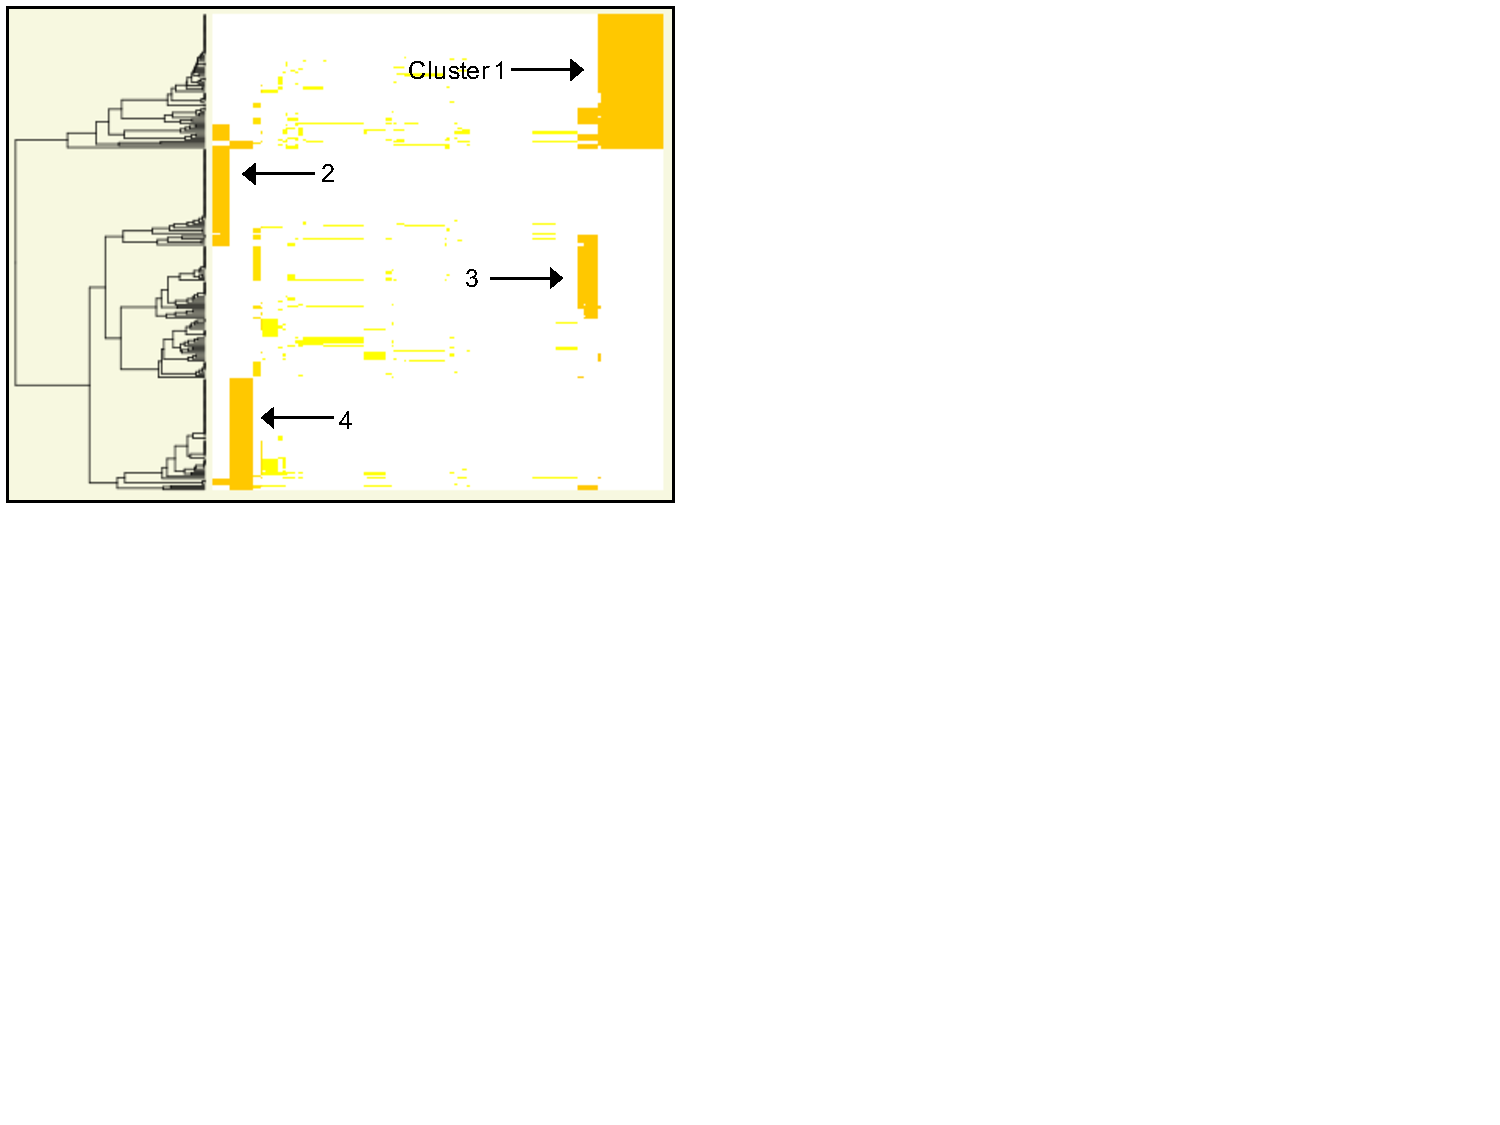
\includegraphics[width=1\textwidth]{chap3figs/figure3_12.pdf}
\caption[Overview heatmap for diseases associated with Unfolded Protein Response.]
{
% Rackham requires the figure list title matches the first sentence, so repeat that sentence here
\textbf{Overview heatmap for diseases associated with Unfolded Protein Response.} Each row represents a MeSH disease and each column is a compound. The UPR is associated with four main groups of diseases, defined by the types of overlapping compounds.  From here, users may click to proceed to an interactive heatmap view.
}
\label{chap3:fig:12}
\end{figure}

\newpage

\begin{figure}[ht!]
\centering
% manually adjust the width of the figure
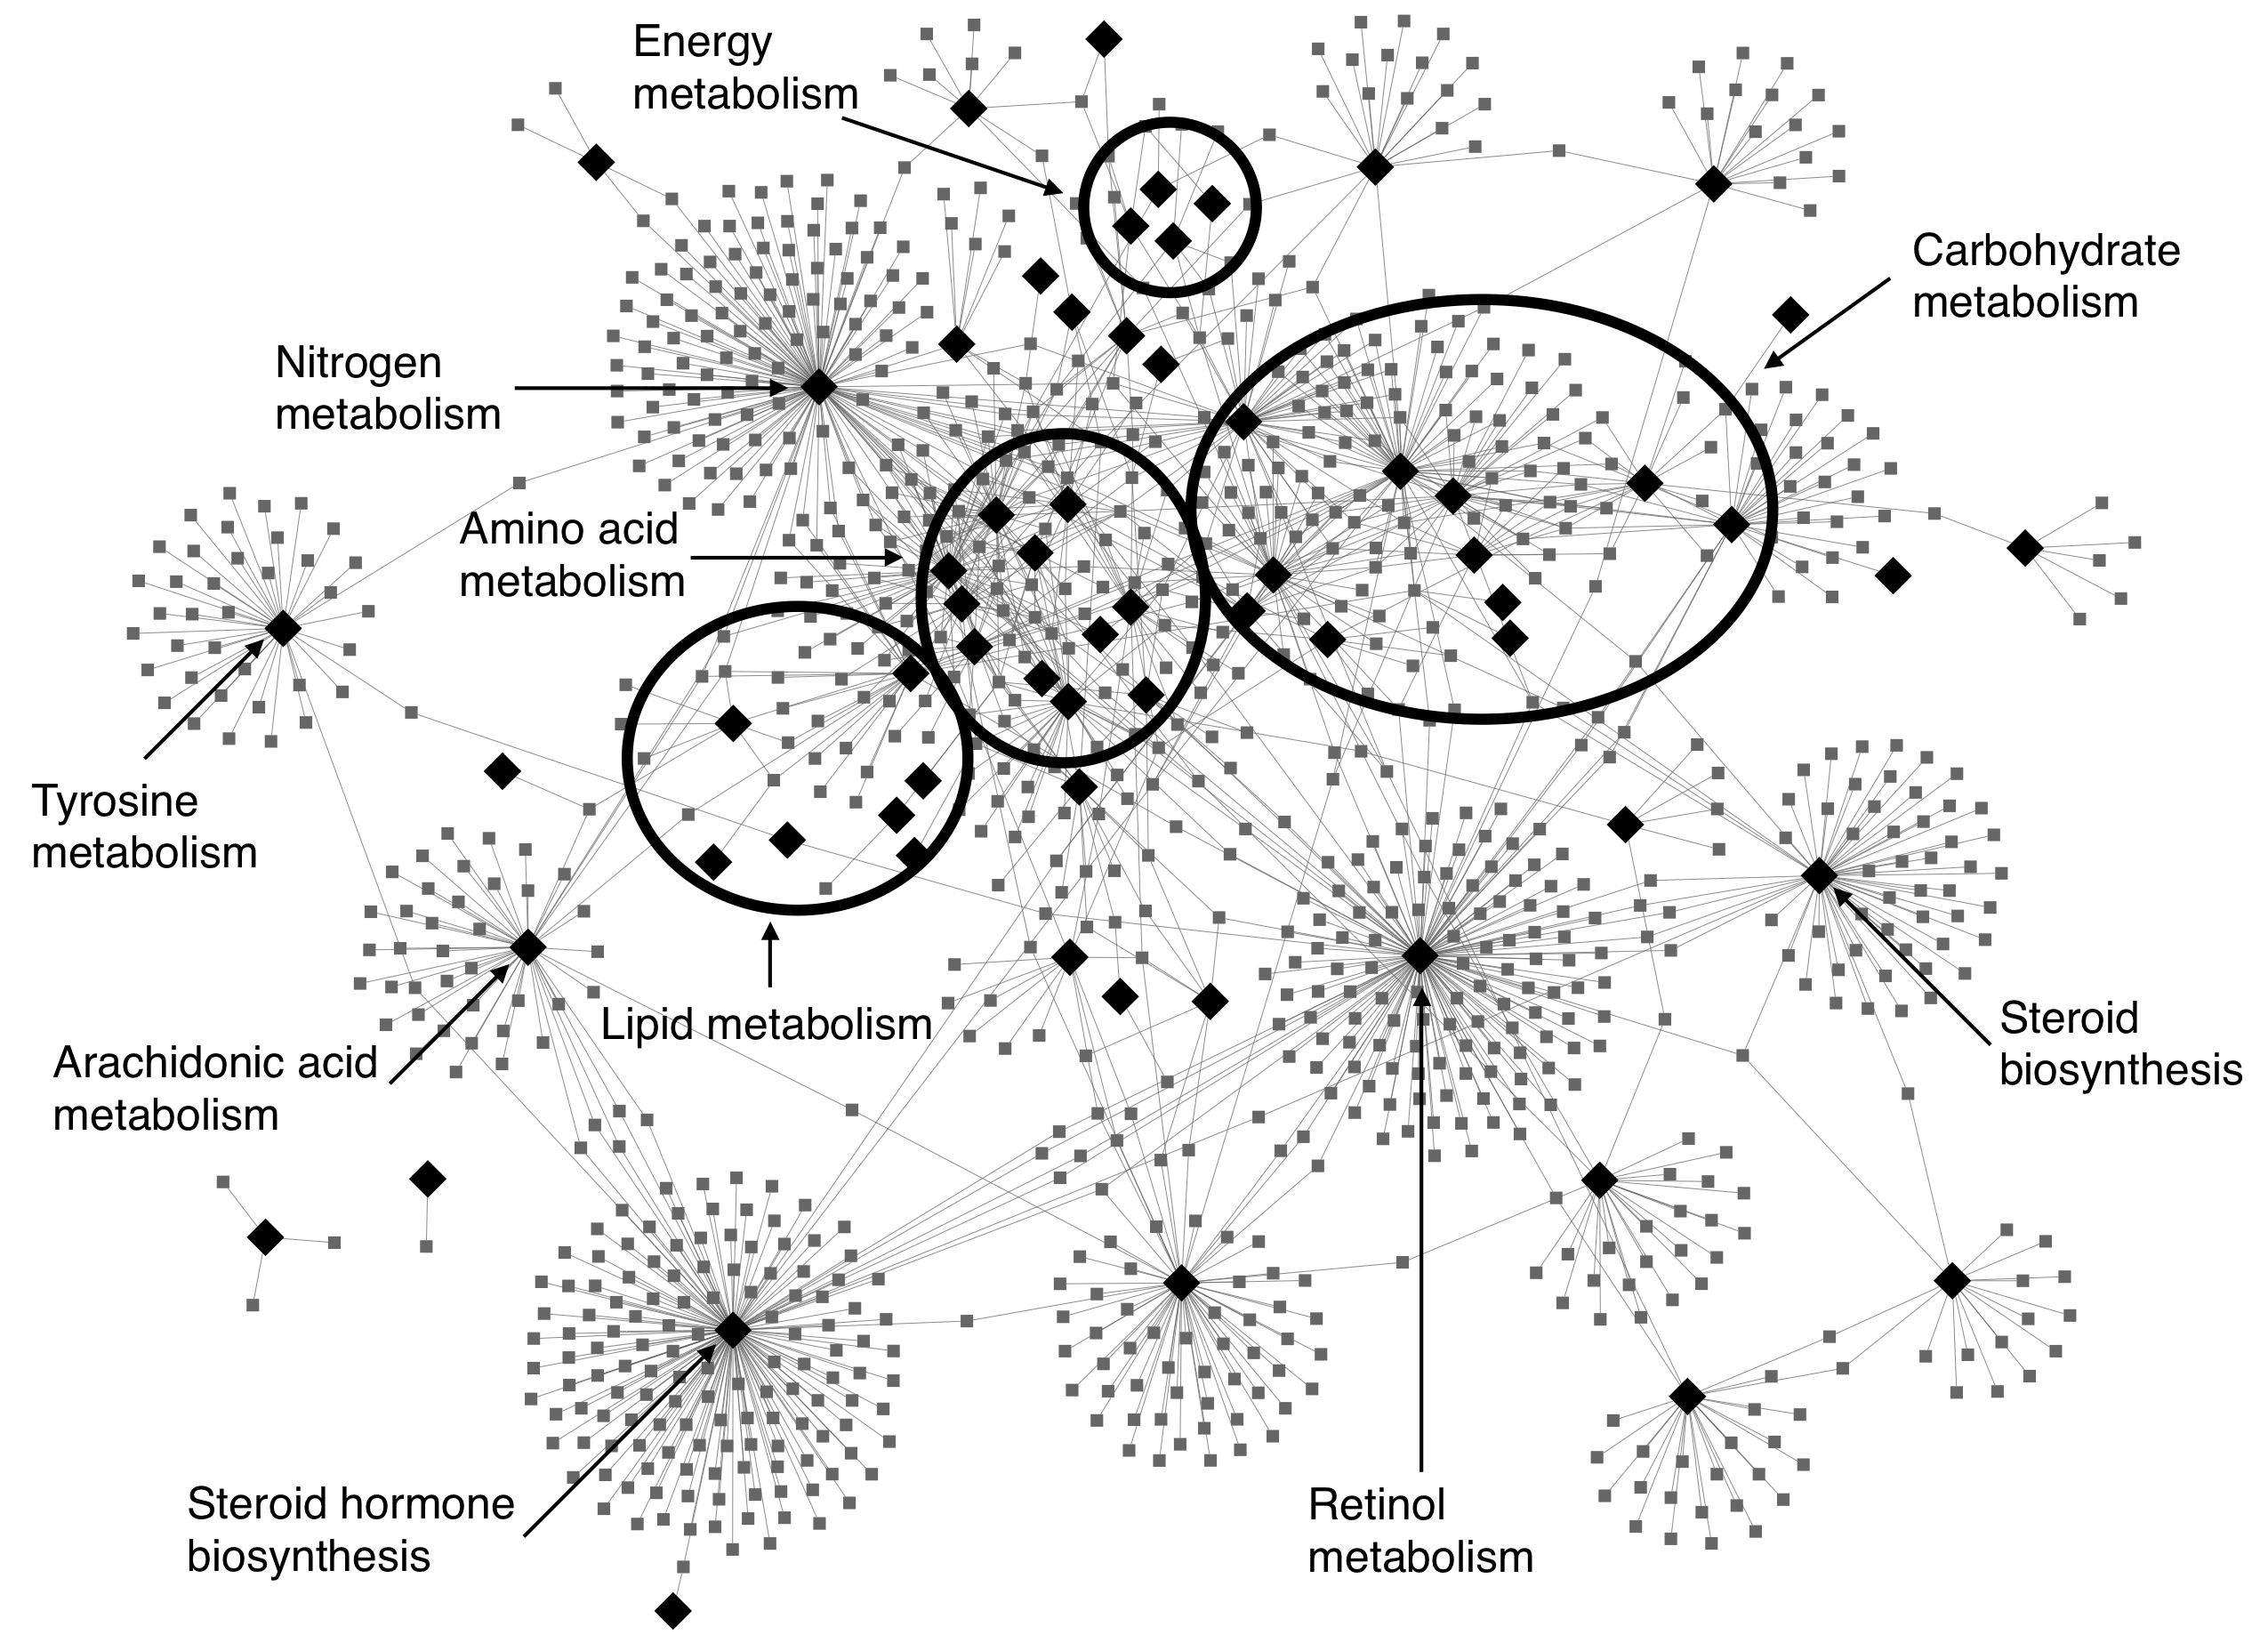
\includegraphics[width=1\textwidth]{chap3figs/figure3_13.jpg}
\caption[Bipartite metabolic pathway.]
{
% Rackham requires the figure list title matches the first sentence, so repeat that sentence here
\textbf{Bipartite metabolic pathway.} A disease network identified by ConceptMetab and displayed in Cytoscape. Black diamonds represent pathways; grey squares are diseases. The ovals in the center represent groups of several KEGG pathways, e.g. carbohydrate metabolism includes amino sugar, nucleotide sugar, galactose, fructose and mannose metabolism.

}
\label{chap3:fig:13}
\end{figure}

\newpage

\begin{figure}[ht!]
\centering
% manually adjust the width of the figure
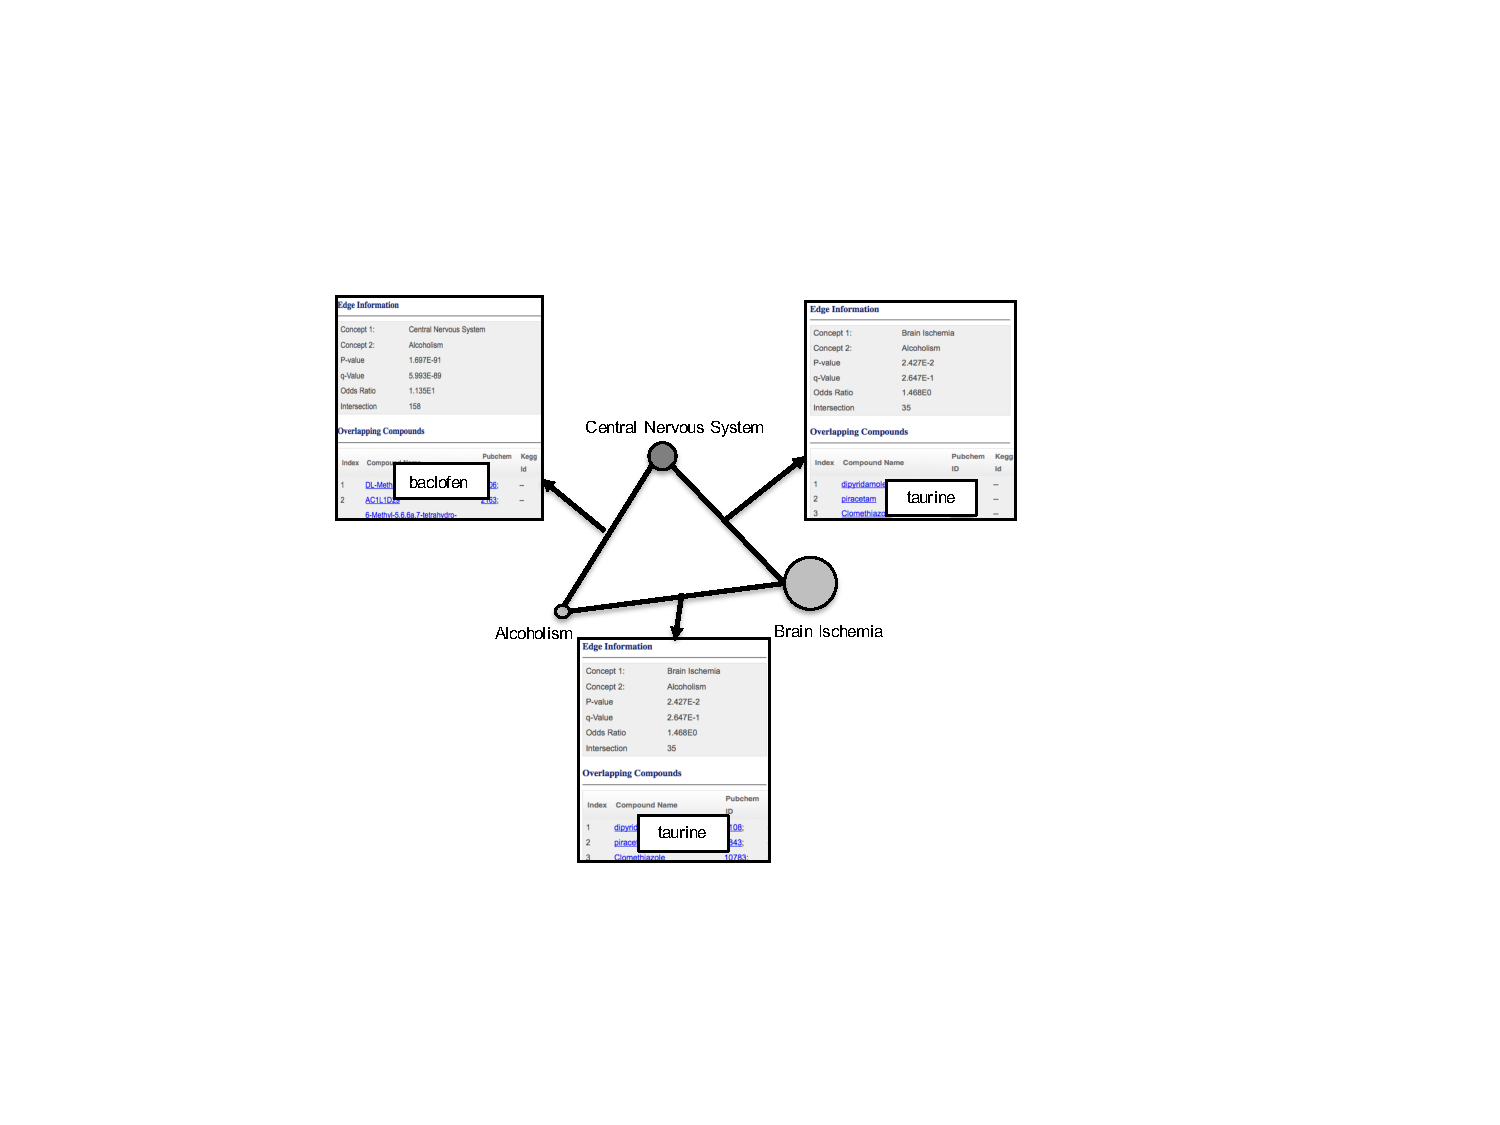
\includegraphics[width=1\textwidth]{chap3figs/figure3_14.pdf}
\caption[ConceptMetab complete network.]
{
% Rackham requires the figure list title matches the first sentence, so repeat that sentence here
\textbf{ConceptMetab complete network.} Network nodes represent concepts. By clicking on an edge user can obtain the information about compounds that are in common between concepts.

}
\label{chap3:fig:14}
\end{figure}
